% Compile with pdflatex -shell-escape base64_encoding.tex
\documentclass[convert={density=300,size=1024x768,outext=.png}]{standalone}

\usepackage{adjustbox}
\usepackage{xcolor}

\usepackage{tikz}
\usetikzlibrary{decorations.pathreplacing}

% Use sans-serif font
\SetSymbolFont{letters}{bold}{OML}{cmbr}{bx}{it}
\renewcommand{\familydefault}{\sfdefault}

% Better-looking hash sign
\let\oldhash\#%
\DeclareRobustCommand{\#}{\adjustbox{valign=B,totalheight=.57\baselineskip}{\oldhash}}%

% Define colors
\definecolor {orange} {RGB}{253, 173, 011}
\definecolor {blue}   {RGB}{131, 223, 238}
\definecolor {green}  {RGB}{162, 250, 163}

\begin{document}
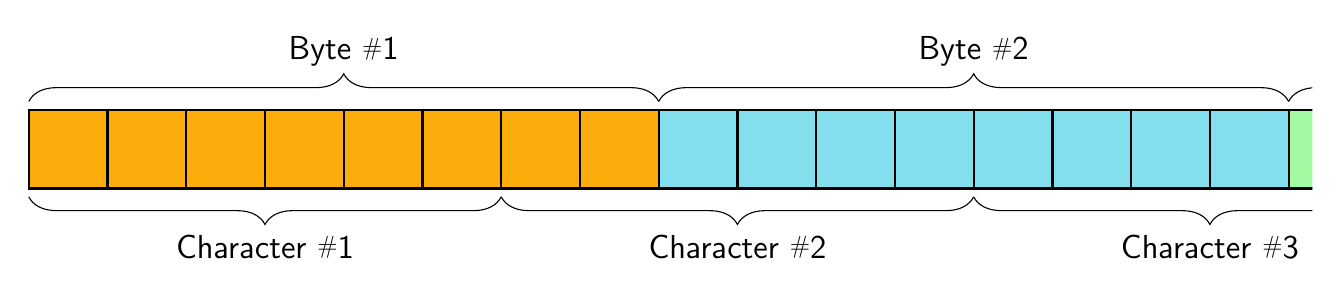
\begin{tikzpicture}

	% Draw boxes corresponding to bytes
	\foreach {\x} in {0, ..., 8}
		\filldraw[thick, stroke=black, fill=orange] (\x, 0) rectangle (\x + 1, 1);

	\foreach {\x} in {8, ..., 15}
		\filldraw[thick, stroke=black, fill=blue] (\x, 0) rectangle (\x + 1, 1);

	\begin{scope}
		\clip (15.9, -0.1) rectangle (16.3, 1.1); % include stroke thickness
		\filldraw[thick, stroke=black, fill=green] (16, 0) rectangle (17, 1);
	\end{scope}

	% Draw curly braces
	% for bytes
	\draw [decorate, decoration={brace, amplitude=10pt}, yshift=+3pt] (0, 1) -- (8, 1) node [black, midway, yshift=+18pt] {\large Byte \#1};

	\draw [decorate, decoration={brace, amplitude=10pt}, yshift=+3pt] (8, 1) -- (16, 1) node [black, midway, yshift=+18pt] {\large Byte \#2};

	\begin{scope}
		\clip (16, 1) rectangle (16.3, 2);
		\draw [decorate, decoration={brace, amplitude=10pt}, yshift=+3pt] (16, 1) -- (24, 1) node [black, midway, yshift=+18pt] {\large Byte \#3};
	\end{scope}


	% for characters
	\draw [decorate, decoration={brace, amplitude=10pt, mirror}, yshift=-3pt] (0, 0) -- (6, 0) node [black, midway, yshift=-18pt] {\large Character \#1};

	\draw [decorate, decoration={brace, amplitude=10pt, mirror}, yshift=-3pt] (6, 0) -- (12, 0) node [black, midway, yshift=-18pt] {\large Character \#2};

	\begin{scope}
		\clip (12, 0) rectangle (16.3, -1);
		\draw [decorate, decoration={brace, amplitude=10pt, mirror}, yshift=-3pt] (12, 0) -- (18, 0) node [black, midway, yshift=-18pt] {\large Character \#3};
	\end{scope}

\end{tikzpicture}
\end{document}
